%% template.tex - Template for a snapshot of modern mathematics from Oberwolfach.
%
% The following authors contributed to this work (in alphabetical order):
%   Carla Cederbaum (concept, testing)
%   Helmut Kastenholz (programming)
%   Konrad Renner (design)
%   Christian Stussak (programming)
%
% with additional support by
%   Sophia Jahns (testing)
%   Christoph Knoth (design)
%   Andreas Daniel Matt (concept)
%   Lea Renner (testing)
%
% To the extent possible under law, the author(s) have dedicated all copyright
% and related and neighboring rights to this software to the public domain worldwide.
% This software is distributed without any warranty. 
%
% You should have received a copy of the CC0 Public Domain Dedication along with
% this file. If not, see <http://creativecommons.org/publicdomain/zero/1.0/>. 
%
%%

%%% Please use pdflatex for compiling this file.
\documentclass{snapshotmfo}

%%%%%%%%%%%%%%%% WILL BE FILLED OUT BY THE EDITORS ACCORDING TO YOUR SPECIFICATIONS %%%%%%%%%%%%%%%%%%%%%%
%\categorizationmath{algebra and number theory,analysis,discrete mathematics and foundations,geometry and topology,numerics and scientific computing,probability theory and statistics} %at least one must be chosen. 
%\categorizationconnect{chemistry and earth science,computer science,engineering and technology,finance,humanities and social sciences,life science,physics,reflections on mathematics} %can be void.
%\license{CC-BY-SA-4.0} %recommended
%\license{CC-BY-ND-4.0}
%\license{CC-BY-NC-SA-4.0} 
%\snapshotid{id}{year}
%\translator{german}{Trans Lator}
\junioreditor{will be filled out by the editors}{junior-editors@mfo.de}
\senioreditor{Carla Cederbaum}{senior-editor@mfo.de}
\director{Gerhard Huisken}
% \junioreditor{First Editor and Second Editor}{junior-editors@mfo.de} "and" will yield the plural "Editors" (Similar for the word "und" in german snapshots).
% With german snapshots the optional argument f for female and m for male of \junioreditor,
% \senioreditor and \director, resp., will make the caption gender-specific, e.g.
% \junioreditor[f]{Anne Schuster}{schuster@example.org} will yield "Editorin ..." instead of "Editor/in ..." and
% \junioreditor[m]{Martin Schuster}{schuster@example.org} will yield "Editor ..." instead of "Editor/in ...".

% Uncomment the following line for snapshots submitted before 2017:
%\logoversionone

%%% Commands for editing
% Uncomment for collaborative editing:
%\usepackage{trackchanges}
%\addeditor{Johannes}
% Uncomment for proofreading:
%\overfullrule=5pt
%%%%%%%%%%%%%%%%%%%%%%%%%%%%%%%%%%%%%%%%%%%%%%%%%%%%%%%%%%%%%%%%%%%%%%%%%%%%%%%%%%%%%%%%%%%%%%%%%%%%%%%%%%


%%%%%%%%%%%%%%%% PLEASE FILL OUT THE FOLLOWING ITEMS %%%%%%%%%%%%%%%%%%%%%%%%%%%%%%%%%%%%%%%%%%%%%%%%%%%%%

%%% Optional recommended packages
%%% Encoding
\usepackage[utf8]{inputenc}
%%% AMS mathematical facilities:
\usepackage{amsmath,amssymb}
%\usepackage{mathtools}
%%% Consistent quotation marks and citations:
%\usepackage{csquotes}
%%% Enhanced typesetting of units:
%\usepackage{siunitx}  
%\sisetup{per-mode=fraction,fraction-function=\nicefrac}
%%% Wrap text around tables and figures:
%\usepackage{wrapfig}

% Please feel free to use your own macros but please do not change the layout of the snapshot.

%%% Please select 'ngerman' instead of 'USenglish' if you want to submit your snapshot in German. If you do choose 'ngerman', please run your LaTeX compiler *twice* or delete the .aux file.
%\usepackage[ngerman]{babel}
\usepackage[USenglish]{babel}

%%% Please separate your names by \and if there are several authors.
\author{Author One\thanks{Author One is supported by the Mathematical Dreams Come True Foundation.} \and Author Two}

%%% Please insert the title of your snapshot.
\title{Your title}

%%% Please provide some information on the author(s).
\authorinfo{\authorname{Author One} is a professor of pure mathematics at the First University.}
\authorinfo{\authorname{Author Two} is a lecturer in applied mathematics at the Second Institution.}


%%%%%%%%%%%%%%%% BIBLIOGRAPHY %%%%%%%%%%%%%%%%%%%%%%%%%%%%%%%%%%%%%%%%%%%%%%%%%%%%%%%%%%%%%%%%%%%%%%%%%%%%
%%% There are three ways to provide your references:
%%% 
%%% 1. by using the embedded .bib file:
%%%    * replace the references below by your own ones
%%%    * and leave the \bibliography command at the end of this file unchanged.
%%% This is the default way as it is a full-fledged BibTex solution
%%% while you have to edit only one file.
%%% 
%%% 2. by using a separate .bib file:
%%%    * provide your own .bib file,
%%%    * delete everything from \usepackage{filecontents} until \end{filecontents}
%%%    * and make the \bibliography command at the end of this file point to your .bib file.
%%% 
%%% 3. by using no BibTeX at all:
%%%    * delete everything from \usepackage{filecontents} until \end{filecontents}
%%%    * replace the \bibliography command at the end of this file with the
%%%      thebibliography environment containing a \bibitem command for each reference.
%%% This way is deprecated as it is less flexible than the BibTeX solutions.
%%%
\usepackage{filecontents}
\begin{filecontents}{\jobname.bib}
@book{knuth1984texbook,
  title = {The TeXbook},
  author = {Knuth, D. E.},
  year = {1984},
  edition={1},
  publisher = {Addison-Wesley},
  isbn = {978-0201134483}
}

@article{snapshot,
  title = {The first snapshot},
  author = {Jahns, S. and Renner, L.},
  journal = {Snapshots of modern mathematics},
  volume = {1},
  number = {1},
  pages = {1--10},
  year = {2014},
  publisher = {MFO}
}

@misc{wikiMath,
  author = {Wikipedia},
  title = {Mathematics --- {W}ikipedia{,} The Free Encyclopedia},
  year = {2014},
  url = {https://en.wikipedia.org/wiki/Mathematics},
  urldate = {2014-05-19}
}

@misc{sample13,
  author = {Sample, J.},
  howpublished = {\href{http://arxiv.org/abs/8765.4321v1}{arxiv:8765.4321v1}},
  title = {Interesting facts in mathematics},
  year = {2013}
}

@incollection{sample12,
  author = {Sample, J.},
  title = {Things you don't know about mathematics},
  booktitle = {A bookseries about mathematics},
  publisher = {Some publisher},
  year = {2012}
}

@inproceedings{sample11,
  author={Example, C.},
  title={A new perspective on mathematics},
  booktitle={New perspectives on arts and sciences},
  year={2011}
}

@phdthesis{sample14,
  author={Candidate, A.},
  title={Thesis title},
  school={MFO},
  year={2014}
}
\end{filecontents}
%%%%%%%%%%%%%%%%%%%%%%%%%%%%%%%%%%%%%%%%%%%%%%%%%%%%%%%%%%%%%%%%%%%%%%%%%%%%%%%%%%%%%%%%%%%%%%%%%%%%%%%%%%


%%%%%%%% If your latex file does not compile, please delete all .aux and .log files and try again. %%%%%%%
\begin{document}

%%% Please insert your abstract here. 
\begin{abstract}[Plain text abstract used as PDF meta data (optional)]
This is your abstract. It should give a brief overview of your snapshot. If possible, please do not use formulas in your abstract. Otherwise, please suggest an additional plain text abstract in square brackets, that can be used in the PDF's metadata field. Please do not use more than 500 symbols.
\end{abstract}

\section{Comment on test-template.tex}
template.tex and test-template.tex differ only by this section!
After three or more compilations of this file the following warnings will remain:
\begin{verbatim}
LaTeX Warning: Overwriting file `./test-template.bib'.
Class snapshotmfo Warning: No snapshot id given.
Class snapshotmfo Warning: No mathematical subject given.
Class snapshotmfo Warning: No connection to other fields given.
Class snapshotmfo Warning: No license information given.
Class snapshotmfo Warning: Unable to compute DOI.

Warning--empty language in sample14
Warning--empty language in sample11
Warning--empty language in snapshot
Warning--empty language in knuth1984texbook
Warning--empty language in sample12
Warning--empty language in sample13
Warning--empty language in wikiMath
\end{verbatim}

With MikTeX on Windows the compilation summary will read:
\begin{verbatim}
LaTeX-Result: 0 Error(s), 6 Warning(s), 2 Bad Box(es), 5 Pages(s)
BibTeX-Result: 0 Error(s), 7 Warning(s)
\end{verbatim}

The ``overwriting file'' warning is ok as long as you provide the references that way.

The ``class snapshotmfo'' warnings will disappear as soon as you supply the expected information.

Do not make the ``empty language'' warnings disappear by supplying a language,
unless you want it explicitely printed in the references!


%%% Please insert the main body of your snapshot here.
\section{A heading}
Your actual snapshot.\footnote{This is a footnote.} As usual, you can give references such as \cite{snapshot, knuth1984texbook, wikiMath, sample13, sample12, sample11, sample14} via the \verb+\cite+ command.\\

We appreciate if you include images or other graphics that illustrate your snapshot. However, please do keep in mind the copyright issues explained in our email in case you include images and graphics you have not produced yourself.

%%% Please use this format to include images. Supported image formats: jpg, pdf, png. Please convert your images to those formats.
\begin{figure}[ht]
        \centering 
        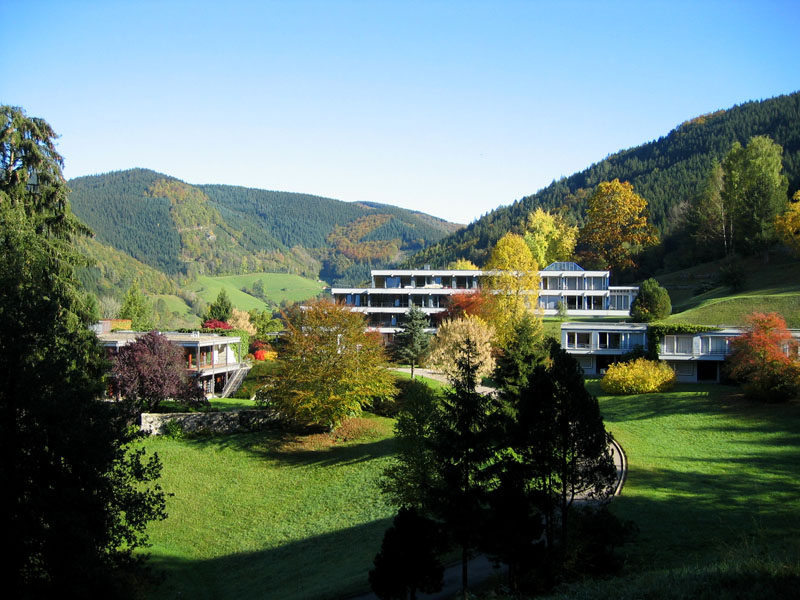
\includegraphics[width= 0.33 \textwidth]{mfo.jpg}
        \caption{An image scaled to 33\% of the textwidth.}
\label{fig:sample-image}
\end{figure}

\subsection{A subsection}
More text and some formulas:
\begin{align}\label{real}
1+1&=2,\\\label{char.2}
1+1&=0.
\end{align}
Formula \eqref{real} refers to $\mathbb{R}$, formula \eqref{char.2} does not.

\section{More information}
We have composed guidelines to help you write a beautiful and accessible snapshot which you can download at \href{http://www.mfo.de/snapshots/guidelines-for-snapshots}{www.mfo.de/snapshots/guidelines-for-snapshots}. For more information on the snapshot project (including example snapshots), please see \href{http://www.mfo.de/snapshots}{www.mfo.de/snapshots}.

%%% Please use this format to include images. Supported image formats: jpg, pdf, png. Please convert your images to those formats.
\begin{figure}[ht]
        \centering 
        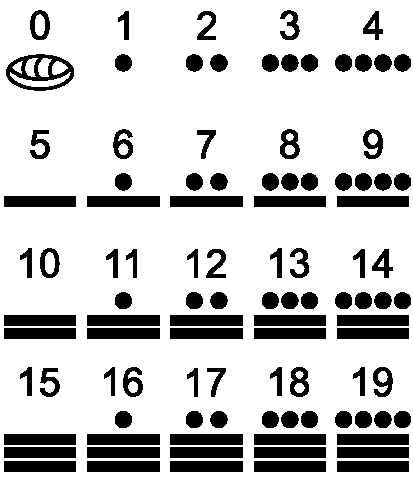
\includegraphics[width= 0.33 \textwidth]{maya.pdf}
        \caption{Exemplary image: Maya numerals.}
\label{fig:maya}
\end{figure}

If you download an image from Wikipedia or similar sources, please always check the applicable license terms. Most licenses require an adequate attribution. For Wikipedia, you can find the correct reference by clicking on the image and then clicking on the button saying 'use this file‘. Some licenses may have further restrictions, such as 'modifications are not allowed'. If modifications are allowed you may still have to mark those modifications. Please verify that you comply with all license requirements.

If you use your own images, please check if you still have the rights of use. The images may be copyrighted by your institution or a publisher of your previous publications.
\clearpage

%%% Image credits: If you download an image form Wikipedia or similar sources, please always check the applicable license terms. Most licenses require an adequate attribution. For Wikipedia, you can find the correct reference by clicking on the image and then clicking on the button saying 'More details' and then on the link 'use this file' or similar. Some licenses may have further restrictions, such as 'modifications are not allowed'. If modifications are allowed you may still have to mark those modifications. Please verify that you comply with all license requirements. If you use your own images, please check if you still have the rights of use. The images may be copyrighted by your institution or a publisher of your previous publications.
\begin{imagecredits}
  \item[Fig. \ref{fig:sample-image}] Archives of the Mathematisches Forschungsinstitut Oberwolfach,\\\url{http://www.mfo.de}, 2004.
  \item[Fig. \ref{fig:maya}] ``Maya''. Author: Bryan Derkson. Licensed under Creative Commons Attribution-Share Alike 3.0 via Wikimedia Commons, \url{http://commons.wikimedia.org/wiki/File:Maya.svg}, visited on September 5, 2014.
\end{imagecredits}

%%%%%%%%%%%%%%%% BIBLIOGRAPHY REVISITED %%%%%%%%%%%%%%%%%%%%%%%%%%%%%%%%%%%%%%%%%%%%%%%%%%%%%%%%%%%%%%%%%%
%%% 1. If you chose to use the embedded .bib file to provide your bibliographical references,
%%% leave the following command unchanged:
\bibliography{\jobname}
%%%
%%% 2. If you chose to use a separate .bib file, make the above command point to it,
%%% e.g. \bibliography{yourbibfile}. Give the file name without the extension .bib.
%%% Please do not forget to *submit* your .bib file together with your .tex file and
%%% your graphics files, if applicable.
%%% 
%%% 3. If you chose to use no BibTeX at all, delete the above \bibliography command
%%% and adopt the following lines as appropriate:
%%%
%\begin{thebibliography}{}
%\bibitem[1]{sample14}A. Candidate, {\slshape Thesis title}, PhD thesis, MFO, 2014.
%\bibitem[2]{sample11}C. Example, {\slshape A new perspective on mathematics}, New perspectives on arts and sciences, 2011.
%\bibitem[3]{snapshot}S. Jahns and L. Renner, {\slshape The first snapshot}, Snapshots of modern mathematics {\bfseries 1} (2014), no.\ 1, 1--10.
%\bibitem[4]{knuth1984texbook}D. E. Knuth, {\slshape The TeXbook}, 1st ed., Addison-Wesley, 1984, ISBN 978-0201134483.
%\bibitem[5]{sample12}J.\ Sample, {\slshape Things you don't know about mathematics}, A bookseries about mathematics, Some publisher, 2012.
%\bibitem[6]{sample13}\underline{\hphantom{J.\ Sam}}\,, {\slshape Interesting facts in mathematics}, arxiv:8765.4321v1, 2013.
%\bibitem[7]{wikiMath}Wikipedia, {\slshape Mathematics --- {W}ikipedia{,} The Free Encyclopedia}, 2014, https://en.wikipedia.org/wiki/Mathematics, visited on May 19, 2014.
%\end{thebibliography}


\end{document}
